
\documentclass{package/notes}
\usepackage[english]{babel}
\usepackage{amssymb,amsmath,amsfonts}  %%% for maths
%%%%%%%%%%%%%%%%%%%%%%%%%%%%%%%%%%%%%
\usepackage{package/color-env}
\usepackage{lipsum}
\usepackage{graphicx}
\renewcommand\qedsymbol{$\blacksquare$}
%%%%%%%%%%%%%%%%%%%%%%%%%%%%%%%%%%%%%

\begin{document}

	\begin{titlepage} % Suppresses headers and footers on the title page
		
		\centering % Centre everything on the title page
		
		\scshape % Use small caps for all text on the title page
		
		\vspace*{\baselineskip} % White space at the top of the page
		
		%------------------------------------------------
		%	Title
		%------------------------------------------------
		
		\rule{\textwidth}{1.6pt}\vspace*{-\baselineskip}\vspace*{2pt} % Thick horizontal rule
		\rule{\textwidth}{0.4pt} % Thin horizontal rule
		
		\vspace{0.75\baselineskip} % Whitespace above the title
		
		{\huge Multivariable Calculus\\} % Title
		
		\vspace{0.75\baselineskip} % Whitespace below the title
		
		\rule{\textwidth}{0.4pt}\vspace*{-\baselineskip}\vspace{3.2pt} % Thin horizontal rule
		\rule{\textwidth}{1.6pt} % Thick horizontal rule
		
		\vspace{2\baselineskip} % Whitespace after the title block
		
		%------------------------------------------------
		%	Subtitle
		%------------------------------------------------
		
		\LARGE{Public Notes for Any Multivariable Calculus Course} 
		
		\vspace*{3\baselineskip} % Whitespace under the subtitle
		
		
		
		\vspace{0.5\baselineskip} 
		
		\vspace{0.5\baselineskip} 
		
		
		\vfill 
		
		%------------------------------------------------
		% Author
		%------------------------------------------------
		
		
		\vspace{0.3\baselineskip} 
		
		
		{\large Edited by\\  Trevor Bushnell} 
		
	\end{titlepage}
	\tableofcontents
%\newpage
\chapter{Vectors and the Geometry of Space}

\section{3D Coordinate Systems}

\subsection{About 3D Coordinate Systems}
	\begin{itemize}
		\item We are used to working in textbf{planes} (1D input and 1D output), and we can model each input and output on a 2D plane
		\item Multivariable calculus is all about representing points in \textbf{space} (2D input and 1D output)
		\item There are 2 \textit{axes} in 2D space $\to$ there are textbf{3 axes} in 3D space
		\item There are 4 \textit{quadrants} in 2D space $\to$ there are 8 \textbf{octants} in 3D space
		\item There is \textit{one plane} in 2D space ($xy$-plane) $\to$ there are \textbf{3 planes} in 3D space ($xy$-plane, $xz$-plane, and $yz$-plane)
		\item Points in 2D space have \textit{2 coordinates} $\to$ points in 3D space have \textbf{3 coordinates}
		\item We went from creating \textit{graphs} in 2D space to creating \textbf{surfaces} in 3D space
		\item If you have a hard time visualizing 3D space, use the room around you and pick a bottom corner in the room
		\begin{itemize}
			\item Floor is $xy$-plane
			\item Left wall is $xz$-plane
			\item Right wall is $yz$-plane
		\end{itemize}
	\end{itemize}

\subsection{The Distance Formula (3D)}

	\begin{itemize}
		\item Distance formula in 3D is very similar to the distance formula in 2D
		\item Finds the distance between point $P_1$ and $P_2$ 
	\end{itemize}

	\newpage
	\begin{definition}[The 3D Distance Formula]{def:label}
		To find the distance between two points $P_1(x_1, y_1, z_1)$ and $P_2(x_2,y_2,z_2)$, use the following distance formula:
		$$D = \sqrt{(x_2-x_1)^2 + (y_2-y_1)^2 + (z_2-z_1)^2}$$
	\end{definition}

\subsection{Equation of a Sphere}
	
	We will be representing many surfaces and it is important to understand the different types of surfaces that we will encounter. A basic one is a sphere, which looks like the following:
	
	\begin{proposition}[The Equation of a Sphere]{prop:label}
	The equation of a sphere with center $C(h,k,l)$ and radius $r$ is
	$$(x-h)^2 + (y-k)^2 + (r-l)^2 = r^2$$
	\end{proposition}


\section{Vectors}

\subsection{About Vectors}

	\begin{definition}[Vectors]{def:label}
		A \textbf{vector} is a quantity that has both a \textit{direction} and a \textit{magnitude} (length).\\

	Ex: 60mph North is a vector because it has a magnitude (60mph) and a direction (North)\\

	We denote a vector by using either boldface ($\mathbf v$) or drawing an arrow over the name of the vector ($\mathbf v$)
	\end{definition}

	\begin{itemize}
		\item $\mathbf{0}$ is called the "zero vector and has length $0$ and no direction
	\end{itemize}

\subsection{Vector Components and Magnitudes}
	\begin{itemize}
		\item A vector algebraically looks like this $\to \mathbf{a} = <a_1, a_2>$ 
		\begin{itemize}
			\item The coordinates of $\mathbf a$ are the \textbf{components} of $\mathbf a$ 
		\end{itemize}
		\item NOTE: Vectors in textbook are represented with boldfont ($\vec{v}$) whereas when handwritten they are expressed with arrows ($\mathbf{v}$) %MARKER
	\end{itemize}

	\newpage
	\begin{proposition}[Vector Components]{prop:label}
		The algebraic representation of a vector between points $A(x_1, y_1, z_1)$ and\\ B$(x_2, y_2,z_2)$ is
		$$\mathbf a = <x_2-x_1,y_2-y_1,z_2-z_1>$$\\

		To find the x-component of a vector, you can use the formula:
		$$\mathbf a_x = ||\mathbf a||\cos\theta$$\\

		To find the y-component of a vector, you can use the formula:
		$$\mathbf a_x = ||\mathbf a||\cos\theta$$\\

		Where $\theta$ is the angle between the vector and the x-axis
	\end{proposition}

	\begin{proposition}[Magnitudes of Vectors]{prop:label}
		To find the magnitude of the vector $\mathbf a$, use the distance formula (2D in the case of working with vectors having 2 components, 3D in the case of working with vectors with 3 components):

		\begin{equation*}
			\begin{aligned}
				||\mathbf a|| =&\: \sqrt {a_1^2 + a_2^2 + a_3^2}\\
				&OR\\
				||\mathbf a|| =&\: \sqrt {a_1^2 + a_2^2}\\
			\end{aligned}
		\end{equation*}
	\end{proposition}

\subsection{Adding Vectors}
	\begin{itemize}
		\item TIP TO TAIL METHOD: Put the end of the second vector on the tip of the first vector \textit{without changing the direction of length}
		\begin{itemize}
			\item The vector connecting the tail of the first vector to the tip of the second vector is the sum of the two vectors
		\end{itemize}
		\item ALGEBRAICALLY: To add two vectors, add together their components
		\item To subtract two vectors, subtract their components
	\end{itemize}

\subsection{Other Properties of Vectors}
	\begin{itemize}
		\item To multiply a vector by a scalar (any number), multiply that scalar by each component of the vector
		\item Other properties of vectors can be found below: 
	
		\begin{figure*}[h]
			\begin{center}
				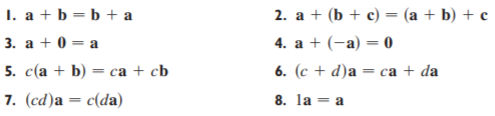
\includegraphics[width=10cm]{images/1.2.1_Image.PNG}
			\end{center}
		\end{figure*}
	\end{itemize}

\subsection{Basis Vectors}
	\begin{itemize}
		\item Vectors can also be written in relation to the unit vectors in the x, y, and z directions respectively (known as the \textbf{basis vectors})
		\item $\mathbf{i} = <1,0,0>$ is the \textbf{basis vector in the $x$-direction}
		\item $\mathbf{j} = <0,1,0>$ is the \textbf{basis vector in the $y$-direction}
		\item $\mathbf{k} = <0,0,1>$ is the \textbf{basis vector in the $z$-direction}
		\item To write up a vector $\mathbf a$ using components, you can add the components of $\mathbf a$ multiplied by the basis vectors
		\begin{itemize}
			\item Ex: $\mathbf a = a_x\mathbf i + a_y\mathbf j + a_z\mathbf k$
		\end{itemize}
	
	\end{itemize}

\subsection{Applications}

	\begin{itemize}
		\item Vectors can be used to represent motion (displacement, position, velocity, acceleration)
		\item Vectors are commonly used to describe \textbf{forces} because all forces are applied with a certain strength (magnitude measure in Newtons) and acting in a certain direction (expressed in angles)
	\end{itemize}



\section{The Dot Product}

\subsection{Definition of the Dot Product}

	\begin{definition}[The Dot Product]{def:label}
		If $\mathbf{a} = <a_1, a_2, a_3>$ and $\mathbf{b} = <b_1, b_2, b_3>$, then the \textbf{dot product of $\mathbf{a}$ and $\mathbf{b}$} is:

		$$\mathbf a \cdot \mathbf b = a_1b_1 + a_2b_2 + a_3b_3$$
	\end{definition}

	\begin{itemize}
		\item The result of a dot product is a \textit{scalar} and \textbf{not a vector}
		\item The dot product obeys many of the laws that hold true for ordinary products
	\end{itemize}

	\begin{proposition}[Physics Definition of the Dot Product]{prop:label}
		If $\theta$ is the angle between the vectors $\mathbf a$ and $\mathbf b$, then $ \mathbf a \cdot \mathbf b = |\mathbf a|\:|\mathbf b |\cos\theta$
	\end{proposition}


\subsection{What Does the Dot Product Represent?}

	\begin{itemize}
		\item Measures the angle between two vectors
	\end{itemize}

	\begin{proposition}[Angle Bweteen Two Vectors]{def:prop}
		The angle between two vectors can be found using the following formula:
		$$\theta = \cos ^{-1}\left(\frac{\mathbf a \cdot \mathbf b}{|\mathbf a | |\mathbf b|}\right)$$
		Where $\theta$ is the angle between vectors $\mathbf{a}$ and $\mathbf{b}$
	\end{proposition}

	\begin{itemize}
		\item Two vectors are \textit{orthogonal} if and only if $\mathbf a \cdot \mathbf b = 0$ 
		\item Dot products also help model the scalar projection of one vector onto another variable
		\end{itemize}

	\begin{proposition}[Scalar Projections]{prop:label}
		Scalar projection of $\mathbf b$ onto $\mathbf a$: $\text{comp}_a b = \frac{\mathbf a \cdot \mathbf b}{|\mathbf a|}$ \\
		Vector projection of $\mathbf b$ onto $\mathbf a$: $\text{proj}_{\mathbf a}\mathbf b = \frac{\mathbf a \cdot \mathbf b}{|\mathbf a|^2}\mathbf a$
	\end{proposition} % Clarify on what this means a little bit more and make sure that I have the terminology correct


\subsection{Direction Angles and Direction Cosines}

	\begin{itemize}
		\item \textbf{DIRECTION ANGLES:} The angles $\alpha, \beta, \gamma$ in the interval $[0,\pi]$ that a vector makes with the positive x, y, or z axes respectively
		\item \textbf{DIRECTION COSINES:} The cosines of the direction angles
	\end{itemize}

	\begin{proposition}[Direction Cosines]{prop:label}
		$$
		\begin{aligned}
			\cos \alpha =& \frac{a_x}{|\mathbf{a}|}\\
			\cos \beta =& \frac{a_y}{|\mathbf a|}\\
			\cos \gamma =& \frac{a_z}{|\mathbf a|}
		\end{aligned}
		$$
	\end{proposition}

	\begin{itemize}
		\item The direction cosines of $\vec a$ are the components of the unit vector in the direction of $\vec a$ 
	\end{itemize}

	\begin{proposition}[Using Direction Cosines to Compute the Unit Vector]{prop:label}
		$$\frac{1}{|\vec a|}\vec a = <\cos\alpha, \cos\beta, \cos\gamma>$$
	\end{proposition}

\section{The Cross Product}

\subsection{Definition of the Cross Product}

	\begin{itemize}
		\item The cross product is another way to multiply vectors
		\item As opposed to a dot product, the cross product returns \textbf{a new vector that is orthogonal to the vectors being crossed}
	\end{itemize}

	\begin{definition}[The Cross Product]{def:label}
		If $\vec a = <a_1,a_2,a_3>$ and $\vec b = <b_1,b_2,b_3>$, then the **cross product of** $\vec a$ and $\vec b$ is:

		$$\vec a \times \vec b = <a_2b_3 - a_3b_2, a_3b_1-a_1b_3, a_1b_2 - a_2b_1>$$

		Instead of memorizing this, an easier way to remember how to compute the cross product is to put the two vectors you wish to cross into a matrix along with the basis vectors and compute the determinant of the 3 x 3 matrix.

		$$
		\vec a \times \vec b = \text{det}\left(\left[
		\begin{array}{ccc}
		\mathbf i & \mathbf j & \mathbf k\\
		a_1 & a_2 & a_3 \\
		b_1 & b_2 & b_3 \\
		\end{array}
		\right]\right)
		$$
	\end{definition}

	\begin{proposition}[Alternate Interpretation of the Cross Product]{prop:label}
		If $\theta$ is the angle between $\vec a$ and $\vec b$ and $0\le\theta\le\pi$, then:
		$$|\vec a \times \vec b | = |\vec a||\vec b| \sin\theta$$
	\end{proposition}

	\begin{itemize}
		\item The cross product is NOT communicative (order matters)
		\item The cross product is NOT associative (parentheses matters)
		\item However, many of the other usual laws of algebra *do* hold for cross products
	\end{itemize}

\subsection{What Does the Cross Product Represent?}

	\begin{itemize}
		\item The magnitude of the cross product of two vectors is the area of the parallelogram that spans between the two vectors being crossed
		\item You can use the right-hand rule to determine the direction of the resultant vector
		\begin{itemize}
			\item If you point your index finger away from you and your middle finger to the left, your thumb  naturally points upward which is the direction of the cross product
		\end{itemize}
		\item Two vectors are parallel if and only if $\vec a \times \vec b = \vec 0$ 
	\end{itemize}

\subsection{Scalar Triple Products}

	\begin{itemize}
		\item \textbf{SCALAR TRIPLE PRODUCT:} The product $\vec a \cdot (\vec b \times \vec c)$ 
		\item \textit{VISUALIZATION:} If considering the parallelepiped determined by the span of vectors $\vec a, \vec b, \vec c$, then the magnitude of the scalar triple product is the volume of the parallelepiped
		\begin{itemize}
			\item In symbols: $V = |\vec a \cdot (\vec b \times \vec c)|$
			\item The visualization makes sense because the area of the base is a parallelogram (meaning the area is the magnitude of the cross product of $\vec c$ and $\vec b$) and $\therefore$ the height is equal to $h = |\vec a| |\cos \theta|$ so dot product (need $|\cos\theta|$ because what is $\theta>\frac{\pi}{2}$)
			\item If $ V = 0$, then the three vectors are \textbf{coplanar} (they all lie in the same plane)
		\end{itemize}
	\end{itemize}

\subsection{Application: Torque}

	\begin{itemize}
		\item \textbf{TORQUE:} The force exerted to produce a turning effect
	\end{itemize}

	\begin{definition}[Torque]{def:label}
		$$
		\begin{aligned}
			\tau = \vec r \times \vec F&\\
			|\tau| = |\vec r \times \vec F| = |\vec r|&|\vec F|\sin\theta
		\end{aligned}
		$$
		\end{definition}


\section{Equations of Lines and Planes}

\subsection{Lines in 3D}

	\begin{itemize}
		\item To determine a line in 2D, you need two points or a point and a slope
		\begin{itemize}
			\item To determine a line in 3D, you need a point and a direction (vector)
		\end{itemize}
	\end{itemize}

	\begin{definition}[Vector Equation for a Line]{def:label}
		$$\vec r = \vec r_0 + t\vec v$$

		Where $\vec r$ is the position vector of any arbitrary point on the line, $\vec r_0$ is the position vector of a point $P_0(x_0,y_0,z_0)$ on line $L$, $\vec v$ is a vector parallel to the line, and $t$ is a scalar.
	\end{definition}

	\begin{itemize}
		\item If the vector $\vec v$ is written in component form, we can rewrite the vector equation for a line as a set of parametric equations for the line $L$ 
	\end{itemize}

	\begin{definition}[Parametric Equations for a Line]{def:label}
		You can express each component of a line int terms of a common variable (usually defined as $t$). This creates a system of equations all in terms of $t$ that express a given line.

		$$
		\begin{aligned}
			x =& x_0 + at\\
			y =& y_0+bt\\
			z =& z_0+ct
		\end{aligned}
		$$
	\end{definition} % I need to clarify what each of the variables mean in this definition

	\begin{definition}[Symmetric Equations for a Line]{def:label}
		These are a set of equations that eliminate the parameter in the parametric equations.

		$$
		\frac{x-x_0}{a}=\frac{y-y_0}{b}=\frac{z-z_0}{c}
		$$

		If one of the parameters $a,b,c = 0$, then we can still write symmetric equations but then we also know in what plane the line lies in. (Ex: if $a= 0$, then the line lies in the plane $x=x_0$)
	\end{definition} % I need to clarify what each of the variables mean in this definition

	\begin{definition}[Line Segments]{def:label}
		The line segment from $\vec r_0$ to $\vec r_1$ is given by the vector equation:

		$$\vec r(t) = (r-t)\vec r_0 + t\vec r_1$$

		Where $t$ lies on the interval from $[0,1]$.
	\end{definition} % Need to go back and review myself wth the standard r means, maybe make a clarification on that

\subsection{Planes}

	\begin{itemize}
		\item A plane in space is determined by a point $P_0(x_0,y_0,z_0)$ in the plane and a vector $\vec n$ that is orthogonal to the plane
	\end{itemize}

	\begin{definition}[Vector Equation of a Plane]{def:label}
		$$
		\vec n \cdot \vec r = \vec n \cdot \vec r_0\\
		OR\\
		\vec n \cdot (\vec r - \vec r_0) = 0
		$$
	\end{definition} %Clarify what each of the variables mean

	\begin{definition}[Scalar Equation of the Plane Through Point $P_0$ With Normal Vector $\vec{n}$]{def:label}
		If $\vec n = <a,b,c>$ and $\vec r = <x,y,z>$ and $\vec r_0 = <x_0,y_0,z_0>$, then the equation  of a plane is:

		$$a(x-x_0) +b(y-y_0)+c(z-z_0) = 0$$
	\end{definition}

	\begin{definition}[Linear Equation of a Plane]{def:label}
		$$ax +by+cz+d=0$$
	\end{definition}

	\begin{itemize}
		\item If you have two vectors that lie in the plane, you can take the cross product of those to vectors to find the normal vector of the plane (since the resulting vector from the cross product is orthogonal to 	the vectors being crossed)
		\item The formula for the distance between a point and a plane in the form $ax+by+cz+d=0$ is 
		$$
		D = \frac{|ax_1+by_1+cz_1+d|}{\sqrt{a^2+b^2+c^2}}
		$$
	\end{itemize}



\chapter{Partial Derivatives}



\chapter{Multiple Integrals}



\chapter{Vector Calculus}




\end{document}
.